\section{Datenverarbeitung}\label{sec:Datenverarbeitung}
Die Bewertung des Systemzustands erfolgt über die ermittelung von drei zentralen Kennwerten. Zum muss der Aktuelle Systemzustand ermittelt weerden. Dieser ist eine Momentaufnahme, die innerhalb der Letzen Minute erfasst wird. Dieser bildet das Kernelement der bewertung. Alle weiteren Kennwerte bauen auf dem Aktuellen Systemzustand auf. Im weiteren verlauf wird dieser als \textit{SytemStatus} betietelt. Desweiteren wird aus den aufzeichnungen des \textit{SystesmStatus} der sogenante \textit{HistorySystemStatus} ermittelt. Dieser Liefert eine historische Einsicht in das Nutzungsverhalten des Systems über eine gewisse Zeit. Zuletzt kann über den \textit{HistorySystemStatus} die, in Abschnitt \ref{sec:MTBF} behandelten, Systemzuverlässigkeit errechnet werden.

\newpage
\subsection{Health Status Definition}
\begin{wrapfigure}{r}{0.2\textwidth}
    \vspace{-1.2cm}
    \begin{center}
      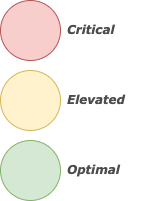
\includegraphics[width=0.2\textwidth]{HealthStatus.png}
    \end{center}
    \vspace{-0.5cm}
    \caption{}
    \label{fig:Systemstatus}
    \vspace{-0.5cm}
\end{wrapfigure}
Der Betrieb der Zielplatform wird zunächst in drei Zustände unterteilt. Sind alle Temperatur und die CPU Auslastung in der Norm, so läuft die Platform im \textit{Optimal} bereich. Steigen Temperaturen oder CPU Auslastung, so steigt der Status auf \textit{Elevated}. Erreicht die Temperatur nun grenzwerte die nich überschritten werden dürfen, begibt sich der SystemStatus in den \textit{Critical} Bereich.\\
Der \textit{Systemstatus} wird daher in die drei Zustände \textit{Optimal}, \textit{Elevated} und \textit{Critical} unterteilt. Der SystemStatus kann, wie in  Abbildung \ref{fig:Systemstatus}, nach dem Ampel Prinzip visualisiert.\\
Die Algorithmen zur ermitteung dieser Werte sind unabhängig von der Hardwarekonfiguration der verschiedenen Zielplatformen. Lediglich die verwendeten Daten die den Algorithmen zur verfügung gestellt werden unterscheiden sich für jede Platform. In den folgenden Abschnitten werden die Algorithmen auf die VisuNet FLX Platform ausgelegt. Dabei wird die Architektur so ausgelegt, das sie für alle anderen Platformen verwendbar ist.
  
\subsubsection*{Hardwarekonfiguration der VisuNet FLX Platform}\label{sec:FLXHardwarekonfiguration}
Damit die Ergebnisse der Bewertungsalgorithmen möglichst genau sind, ist es wichtig mit den Richigen Werten zu rechnen. Zum einen müssen die richigen Temperaturgrenzen für das System festgelegt werden. 
\begin{center}
    \begin{figure}[h!]
        \centering
        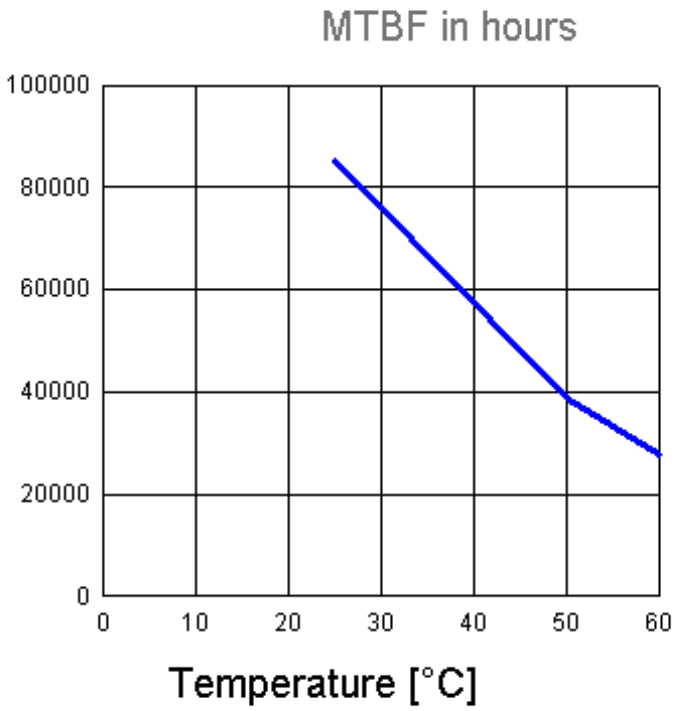
\includegraphics[width=0.3\textwidth]{FLXMTBFPrediction}
        \caption{\ac{mtbf} Voirhersage für die VisuNet FLX Platform}
        \label{fig:FLXMTBF}
    \end{figure}
\end{center}
\vspace{-1.8cm}
Die aus Anhang \ref{app:mtbfprediction} entnommene Abbildung \ref{fig:FLXMTBF} stellt den \ac{mtbf} ,der VisuNet FLX Platform, in Abhängigkeit zur Betriebstemperatur des Gerätes. Aus dieser werden drei Intervalle für den Betrieb des 
Gerätes festgelegt. Von 0°C bis 45°C läuft das Gerät im \textit{Optimal} Betrieb. Dabei wird für dieses Interval eine \ac{mtbf} von 60000h angenommen. Im zweiten Intervall von 45°C bis 63°C läuft das Geräte im \textit{Elevated} betrieb. Der angenommene \ac{mtbf} für dieses Intervall ist 40000h. Bei allem über 63°C läuft das Gerät im \textit{Critical} betrieb, mit einem \ac{mtbf} 30000h.\\
\\
Um die \ac{mtbf} Vorhersage aus Abbildung \ref{fig:FLXMTBF} mit den Temperaturen der Hardware verwenden zu können, müssen hierfür die richtigen Sensoren verwendet werden. Abbuldung \ref{fig:FLXSensoren} Zeigt die Sensorverteilung auf der VisuNet FLX Platform. Da CPU und Spannungsregulator (Siehe Abb. \ref{fig:FLXSensoren} \textit{VR VCC Temperature} und \textit{CPU Temperature}) zwei Signifikante Hitzequellen sind, wird der Sensor \textit{Temperatur 1} zur bestimmung der Betriebstemperatur gewählt. 
\todo{Temperatur 1 typo korregieren}
\begin{center}
    \begin{figure}[h!]
        \centering
        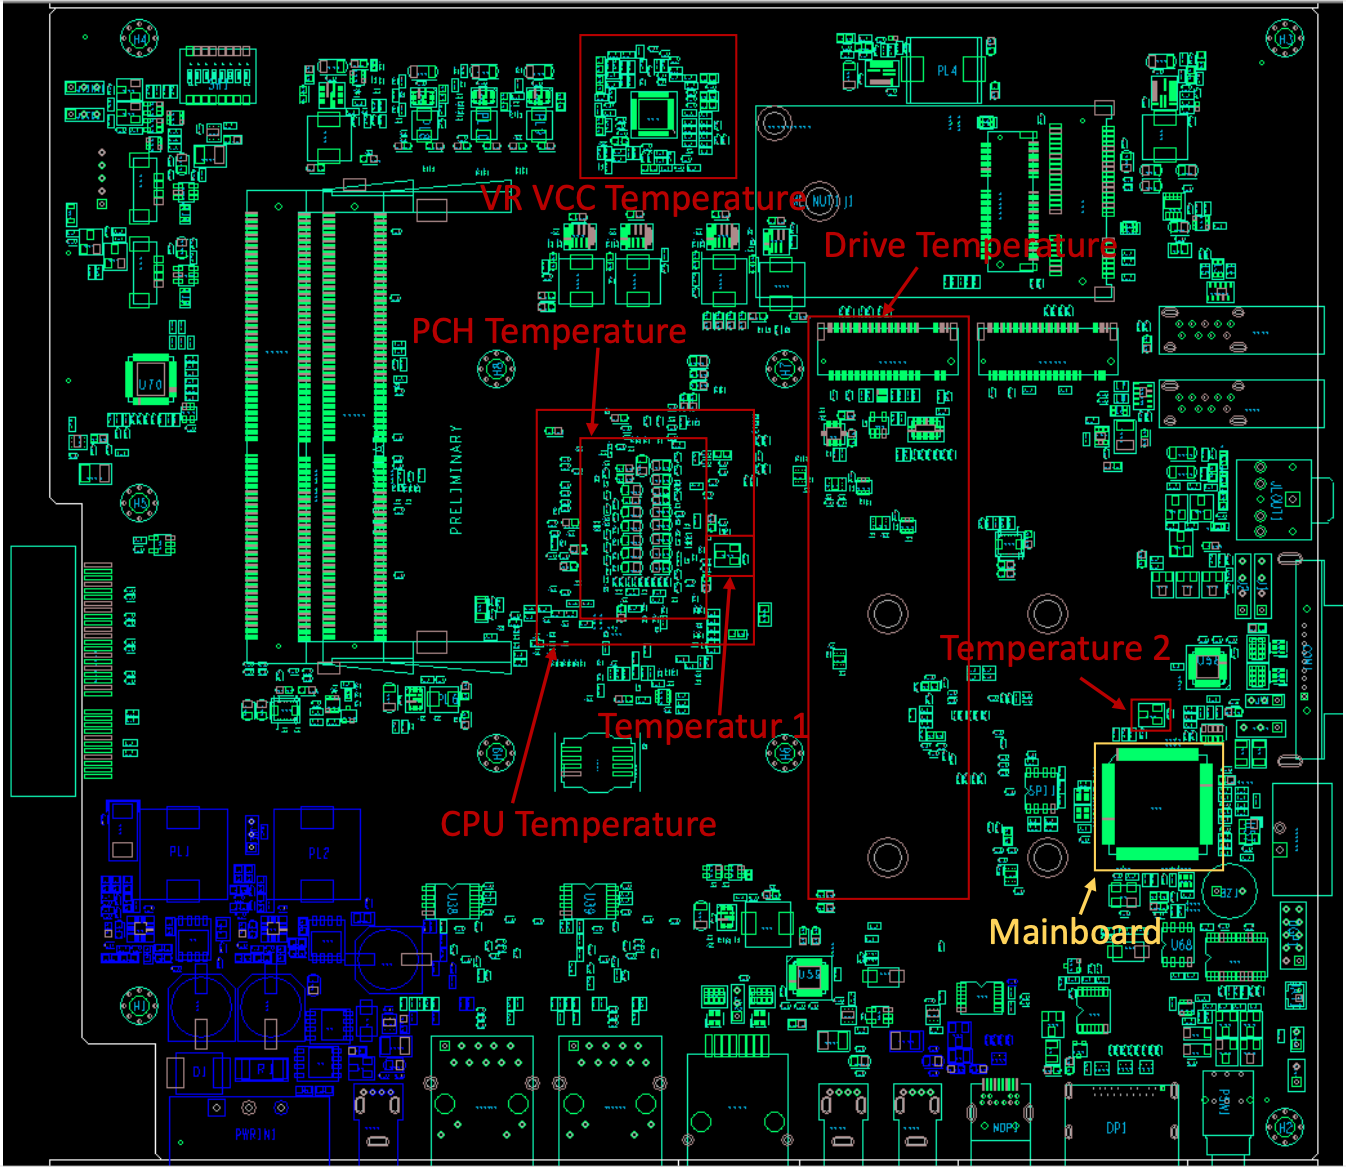
\includegraphics[width=0.8\textwidth]{FLXSensorPlatzierung}
        \caption{Sensorverteilung auf der Mainboard Platine der VisuNet FLX Platform}
        \label{fig:FLXSensoren}
    \end{figure}
\end{center}
\vspace{-1.8cm}  

\subsection{Aulegung einr FuzzyLogic zur Ermittelung des SystemStatus}
Der \textit{SystemStatus} wird mithilfe des, in Abschnit \ref{sec:FuzzyLogic} beschriebenen, FuzzyLogic Verfahren ermittelt. Das System soll dabei so ausgelegt werden, das der \textit{SystemStatus} von Temperatur und CPU Last abhängt.\\
Im ersten Schritt müssen daher zunächst die Linguistischen Variablen, welche die Ein- und Ausgänge der FuzzyEngine representieren, definiert werden. Zu dem müssen auch die passenden Zugehörigkeitsfunktionen definiert werden. Diese sind mathematische Funktionen, welche angeben, wie stark ein Wert zu einem bestimmten Linguistischen Begriff gehört. \cite{FuzzyLogicGeeks}\\ 

\subsubsection*{Definition der linguistische Variablen und der Zugehörigkeitsfunktionen}
Die Temperaturen werden der linguistischen Variable \textit{Temperature} zugeordnet. Zudem werden drei Zugehörigkeitsfunktionen definiert. Diese sind in Abbildung \ref{fig:MSFTemp} abfebildet. Dabei werden die grenzen der Funktionen an die in Abschnitt \ref{sec:FLXHardwarekonfiguration} aufgestellten Temperaturintervalle angepasst. Es werden insgesammt drei Trapezförmige Funktionen erstellt. Die Funktionen werden mit den Begriffen \textit{Low}, \textit{Medium} und \textit{High} Bezeichnet.
\begin{center}
    \begin{figure}[h!]
        \centering
        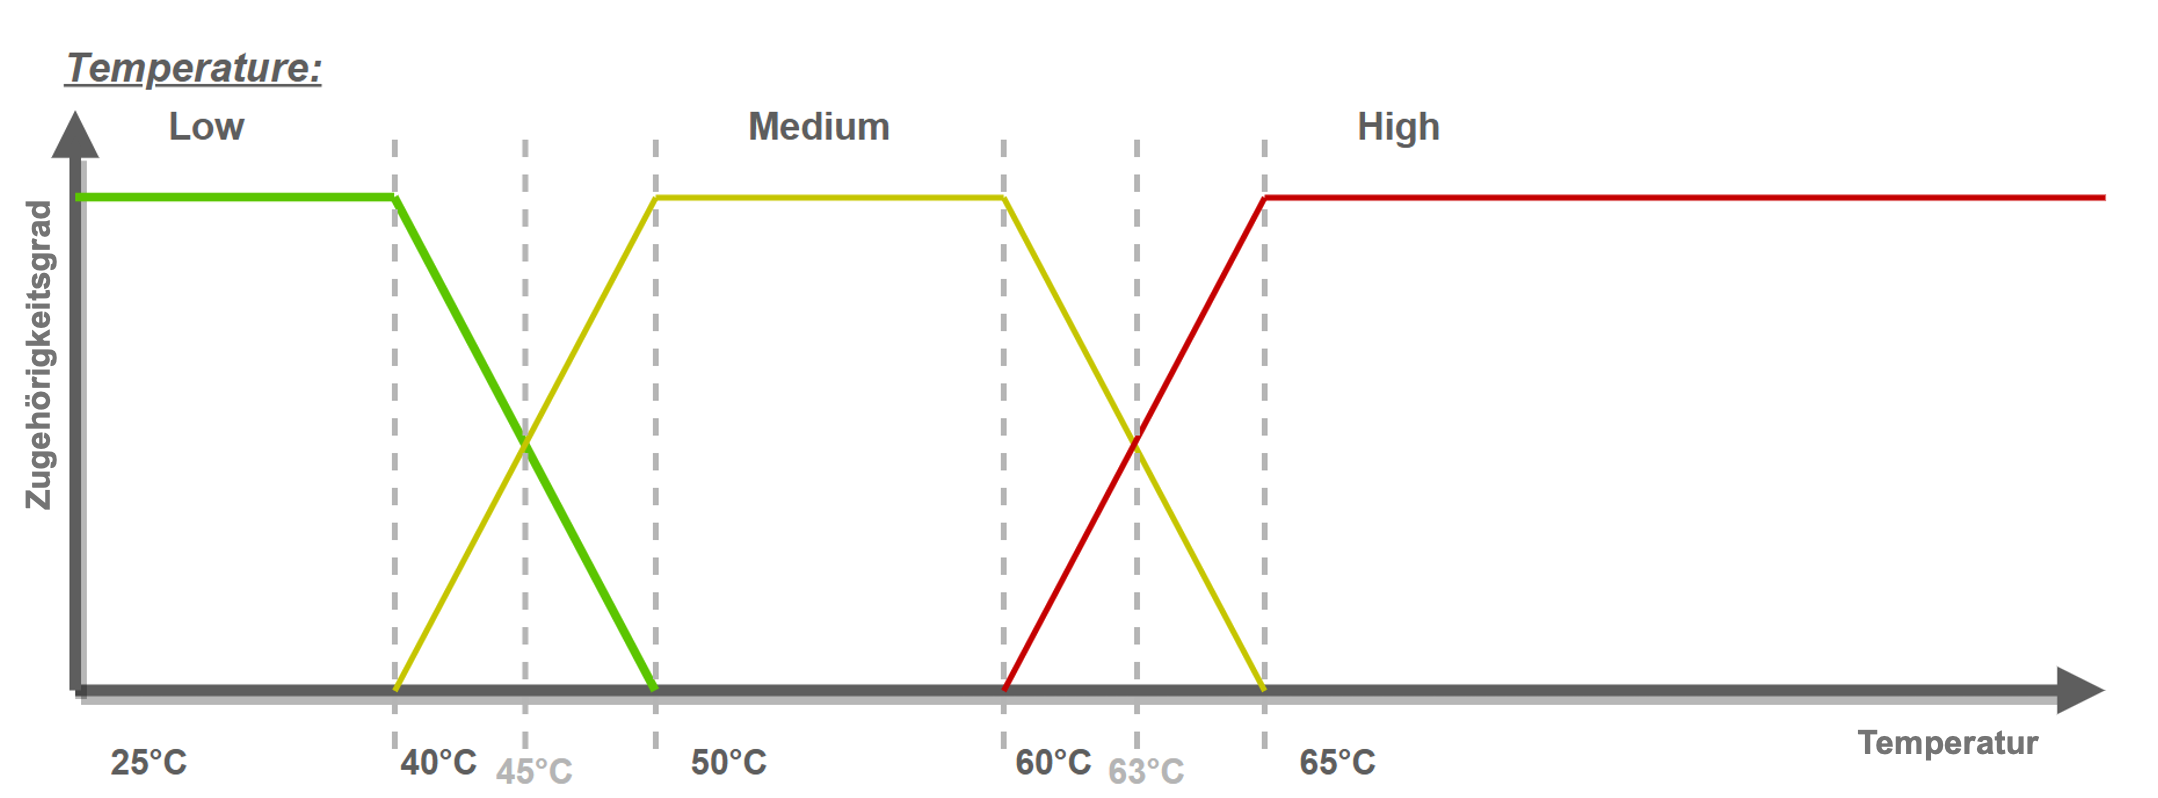
\includegraphics[width=1\textwidth]{MSFTemp.png}
        \caption{Zugehörigkeitsfunktionen der Temperature Variable}
        \label{fig:MSFTemp}
    \end{figure}
\end{center}
\vspace{-0.5cm}
Die Auslastung der CPU wird der linguistischen Variable \textit{CPULoad} zugeordnet. Wie auch bei den Zugehörigkeitsfunktionen der Temperatur, werden hierfür ebenfalls drei Trapezförmige Funktionen aufgestellt. Diese werden ebenfalls mit den Begriffen \textit{Low}, \textit{Medium} und \textit{High} Bezeichnet. Die Zugehörigkeitsfunktionen Funktionen der Variable \textit{CPULoad} werden in Abbildung \ref{fig:MSFCPULoad} dargestellt.
\begin{center}
    \begin{figure}[h!]
        \centering
        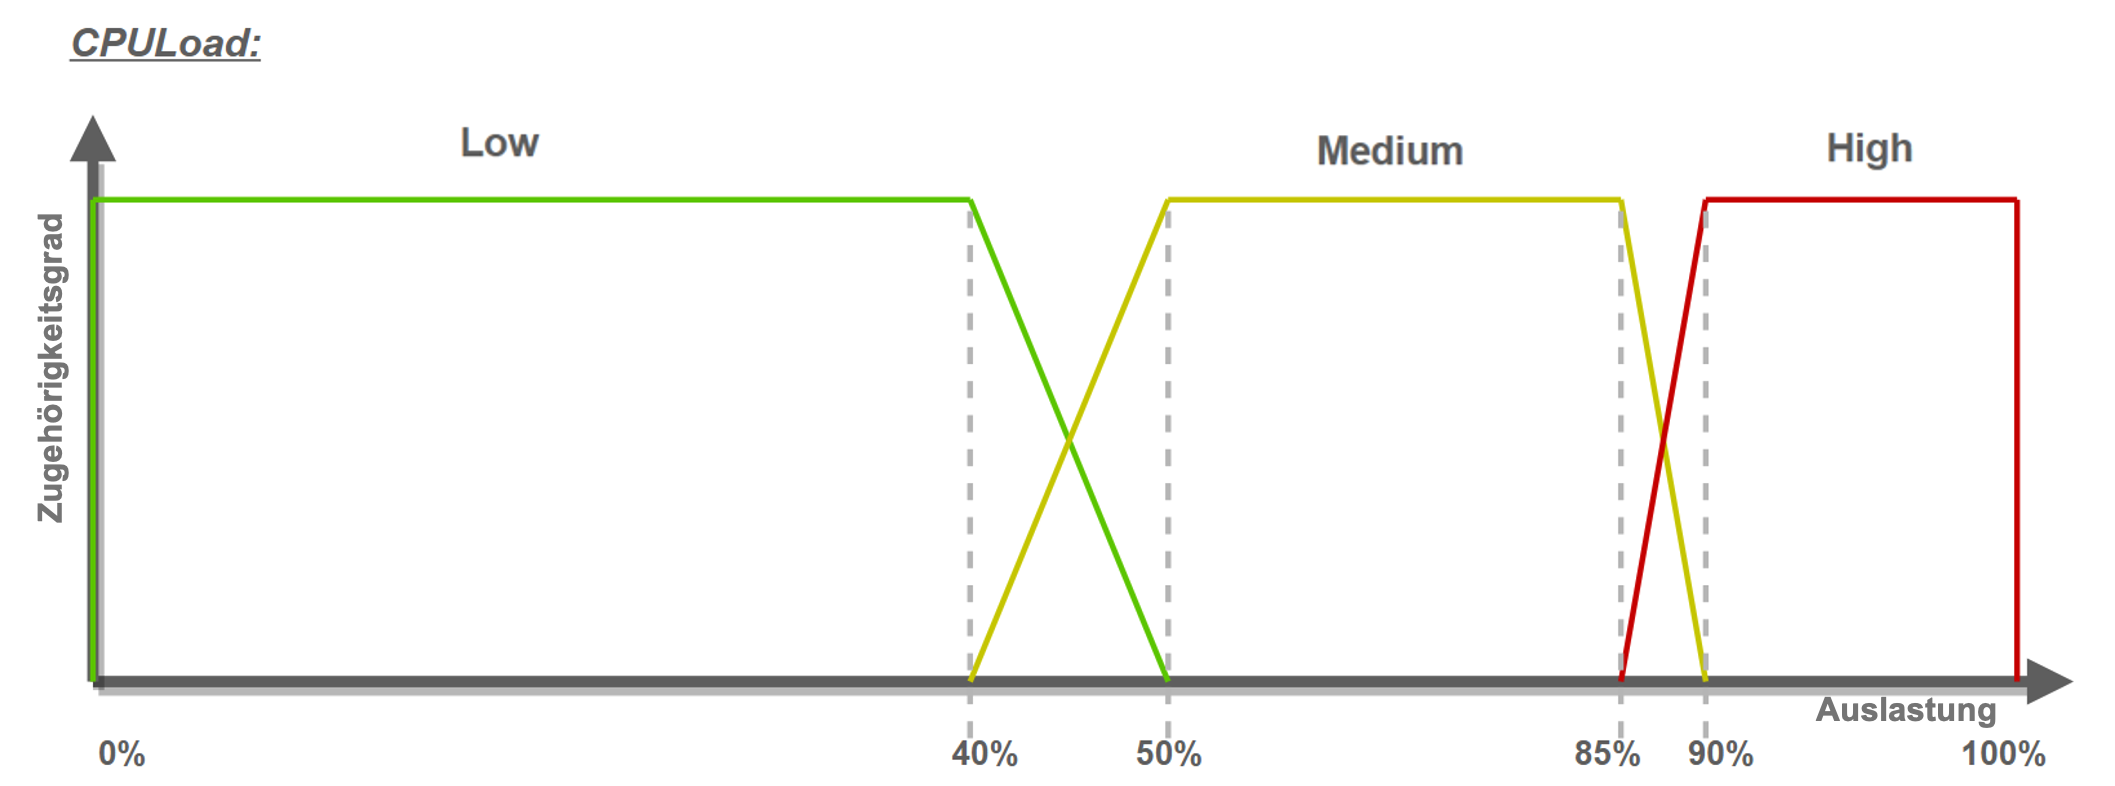
\includegraphics[width=1\textwidth]{MSFCPULoad.png}
        \caption{Zugehörigkeitsfunktionen der CPULast Variable}
        \label{fig:MSFCPULoad}
    \end{figure}
\end{center}
\vspace{-0.5cm}
Der Ausgang der Engine wird als die linguistische Variable \textit{SystemStatus} deklariert. Hierzu werden drei Rechteck Funktionen \textit{Optimal}, \textit{Elevated} und \textit{Critial} erzeugt. Das Ergebniss wird in \% angegeben, wobei jede Funktion genau ein Drittel darstellt. Die Funktionen der \textit{SystemStaus} Variable sind in Abbildung \ref{fig:MSFSystemStaus} dargestellt.
\begin{center}
    \begin{figure}[h!]
        \centering
        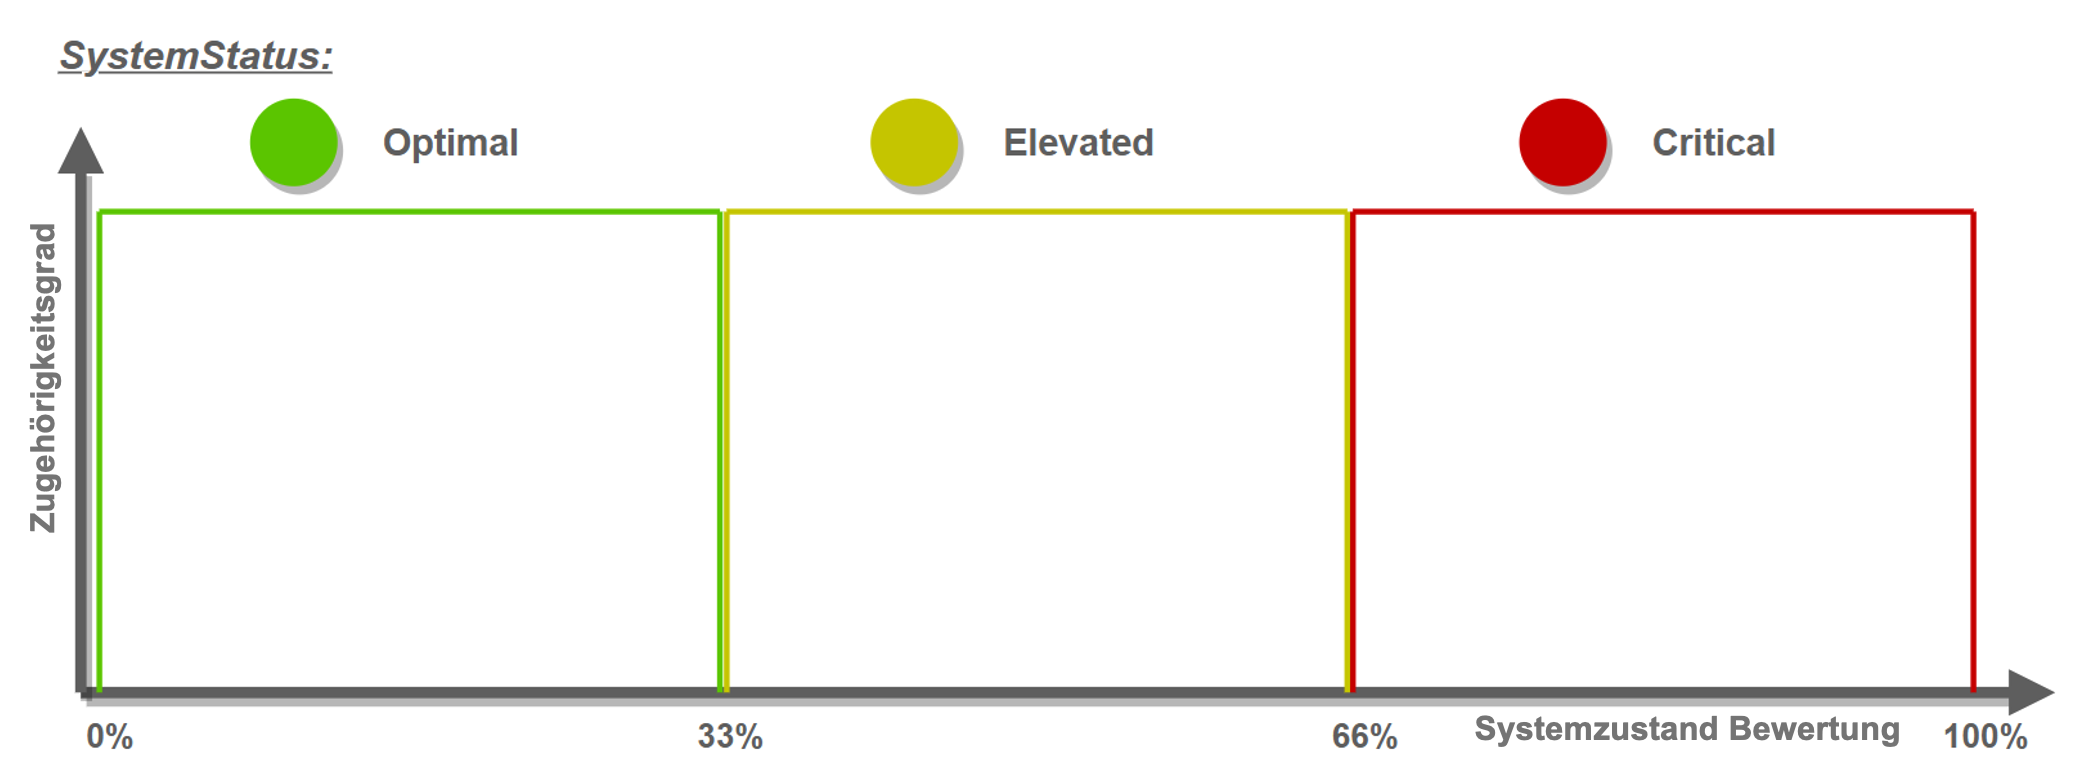
\includegraphics[width=1\textwidth]{MSFSystemStaus.png}
        \caption{Zugehörigkeitsfunktionen der SystemStatus Variable}
        \label{fig:MSFSystemStaus}
    \end{figure}
\end{center}
\vspace{-0.5cm}  

\subsubsection*{Definition der Regeln}
Im zweiten Schritt beim auslegen eines FuzzyLogic Systems muss das Regelwerk festgelegt werden. Die Regeln eines Solchen Systems sind dabei verbal gefasst und drücken die Beziehung zwischen den linguistischen Varbiablen der Ein- und Ausgänge aus.\cite{FLRegelwerk} \\
Die Ausgangsvariable \textit{SystemStatus} wird in abhängigkeit von den Eingangsvariablen \textit{Temperature} und \textit{CPLoad} gesetzt. Dabei werden die möglichen Zustände der Variable, die in Abbildung \ref{fig:MSFSystemStaus} gezeigt werden, wie folgt definiert. 
\begin{enumerate}
    \item \textit{SystemStatus: Optimal}\\
    Das System operiert im \textit{Optimal} bereich, solange die Temperatur des Systems in die wertebereich der Zugehörigkeitsfunktion \textit{Low} fällt. Zudem muss die Auslastung der CPU in im wertebeirechder Zugehörigkeitsfunktion \textit{Low} oder \textit{Medium} liefen.  
    \item \textit{SystemStatus: Elevated}\\
    Das System operiert im \textit{Elevated} bereich, sobald die Temperatur des Systems in den wertebereiche der Zugehörigkeitsfunktion \textit{Medium} oder die Auslastung der CPU in den wertebereich der Zugehörigkeitsfunktion \textit{High} fällt.
    \item \textit{SystemStatus: Critical}\\
    Das System operiert im \textit{Critical} bereich, wenn die Temperatur des Systems in den Werteberiech der Zugehörigkeitsfunktion \textit{High} fällt. Dies bleibt unabhängig von der CPU Auslastung des Systems. 
\end{enumerate}
Aus dieser Zustandsdefinition kann somit das, in Abschnitt \ref{fig:FuzzyLogicRuleBase} gezeigte, Regelwerk zur Ermittelung des Systemzustands abgeleitet werden .  
\begin{center}
    \begin{figure}[h!]
        \centering
        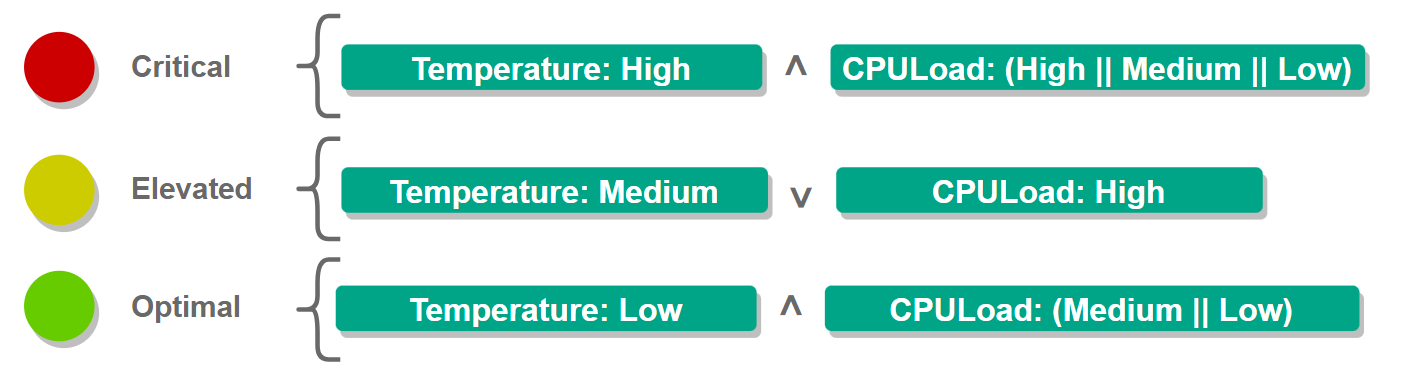
\includegraphics[width=1\textwidth]{RegelWerk.png}
        \caption{Regelwerk Systemstauts}
        \label{fig:FuzzyLogicRuleBase}
    \end{figure}
\end{center}
\vspace{-0.5cm}  

\subsubsection*{Architektur}
Da die Basis der FuzzyLogic für jede Zielplatform die selbe ist, wird zunächst über das \textit{IFuzzyLogic} Interface, die Schnittstelle zur FuzzyEngin definiert. Hierraus wird anschließend die Abstrakte Basisklasse \textit{FuzzyLogic} abgeleitet werden. Diese beinhaltet die verwendeten Linguistischen Variablen, die jeweiligen Zugehörigkeitsfunktionen, so wie die Methoden zum berechnung der Ergebnisse.\\
Aus der \textit{FuzzyLogic} Klasse können Anschließend weitere Klassen abgeleitet werden,in denen die gewünschten Zugehörigkeitsfunktionen für die jeweiligen Zielplatform angelegt werden können. Das in der Basisklasse definierte Regelwerk kann bei bedarf in der Abgeleiteten klasse überschrieben werden. Die Struktur des \textit{HM.ScoringModel} Verzeichnises wird in Abbildung \ref{fig:ScoringModel} visualisiert.  
\begin{center}
    \begin{figure}[h!]
        \centering
        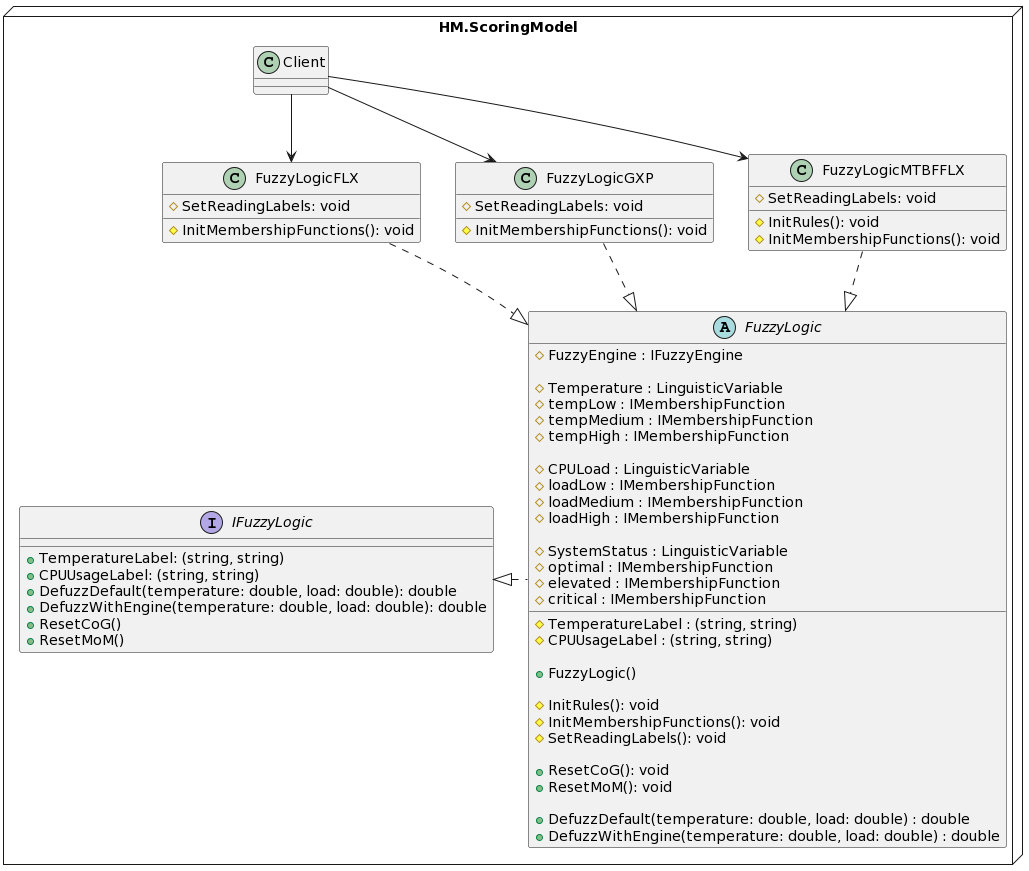
\includegraphics[width=1\textwidth]{ScoringModel.png}
        \caption{Architektur des HM.ScoringModel für die Ermittelung des SystemStatus}
        \label{fig:ScoringModel}
    \end{figure}
\end{center}

\subsection{Ermittelung der Systemstatus Historie und der Systemzuverlässigkeit}
Um die Systemstatus Historie des System zu berechnen, werden die aufzeichnungen des Systemstatus benötigt. Diese müssen im gewünschten Intervall, beispielsweise der letztn 24h, gegeben sein.
Die Idee besteht im wesentlichen daraus, die zeit zwischen zwei Systemzuständen, für jeden zustand \textit{Optimal}, \textit{Elevated} und \textit{Critacal} zu addieren. Somit kommt man auf die Zeiten, in dem das System im jeweiligen Zustand verbracht hat. Anschließend können die einzelnen zeiten duch die gesammte Zeit des Intervals geteilt werden, um auf die prozentualen anteile der jeweiligen Zustände zu kommen.\\
Hierzu visualisiert das in Abbildung \ref{fig:SystemStatusHistoryAlgorythmus} visualisierte ablaufdiagremm, die ermittlung der Systemzusands Historie. Die Systemstatus Historie wird in der \textit{HistorySystemStatus} Tabelle der Datenbank abgespeichert. (Siehe Abbildung \ref{fig:DBModellErweitert})
\begin{center}
    \begin{figure}[h!]
        \centering
        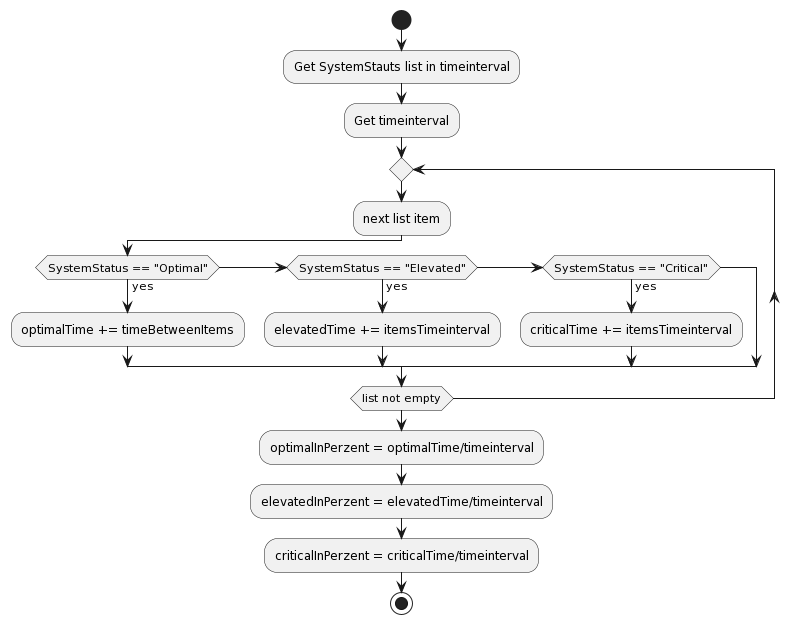
\includegraphics[width=0.87 \textwidth]{SystemStatusHistory.png}
        \caption{Algorithmus zur berechnung der Systemstatus Historie}
        \label{fig:SystemStatusHistoryAlgorythmus}
    \end{figure}
\end{center}
\vspace{-1cm}
Über die in Abschnitt \ref{sec:MTBF} beschrieben Formel \ref{equ:Reliability} kann die  Reliability (Zuverlässigkeit) des Systems berechnet werden. Hierzu wird zum einen die Laufzeit des Systems, zum anderen der temperaturabhängige \ac{mtbf} des Systems benötig. Jedoch kann diese Formel nicht direkt angewendet werden. Zum einen gibt es keine direkte Aufzeichnung über die gesmate Laufzeit des Systems. Zum anderen varriert die Betriebstemperatur des Systems, sodass man für verschiedene Betriebstemperaturen verschiedene \ac{mtbf} Werte verwenden muss.\\
Abhilfe hierzu schaft der Algorithmus zur kalkulation der Systemstatus Historie. Die Idee hinter diesem Ansatz besteht darin, die unterschiedlichen Betriebstemperaturen mithilfe der FuzzyLogic Klasse und einem angepassten Regelwerks aufzuzeichnen. Anschließend kann hierzu die SystemStatus Historie berechnet werden. Das ergebniss liefert somit eine genaue aussage darüber, wie lange das System in welchem Temperaturbereich gearbeitet hat. Somit bekommt man zum einen die Systemlaufzeit, zum anderen den zugehörigen temperaturabhängigen \ac{mtbf} zur berechnung der Systemzuverlässigkeit.\\ 
Um bei der Berechnung der Systemzuverlässigkeit nicht jedes mal alle werten zu benutzen, wird diese zudem nur für eine kleine zeitspanne, beispielsweise alle 24h, erneut durchgeführt. Das Ergebnis kann anschließend mit dem Ergebnis der vorherigen berechnung verrechnet werden, um auf die aktuelle Systemzuverlässigkeit zu kommen.\\
Um die Berechnung durchführen zu können muss daher zunächst das Regelwerk der FuzzyEngin angepasst werden. Hierzu wird die in Abbildung \ref{fig:FuzzyLogicArchitektur} abgebildete Klasse \textit{FuzzyLogicMTBFFLX} mit dem in Abbildung \ref{fig:SystemMTBF} abgebildeten Regelwerk angelegt. Der Ausgang \textit{SystemStatus} so wie der eingang \textit{Temperature}, so wie die korespondierenden Zugehörigkeitsfunktionen bleiben dabei unverändert. (Siehe Abbildung \ref{fig:MSFSystemStaus} und \ref{fig:MSFTemp}). Eingang \textit{CPULoad} fällt weg. Der Zustand des Eingangs wird eins zu eins auf den Ausgang übersetzt. Abbildung \ref{fig:SystemMTBF} veranschaulicht das angepasste Regelwerk der \textit{SuzzyLogicMTBF} Klasse.
\begin{center}
    \begin{figure}[h!]
        \centering
        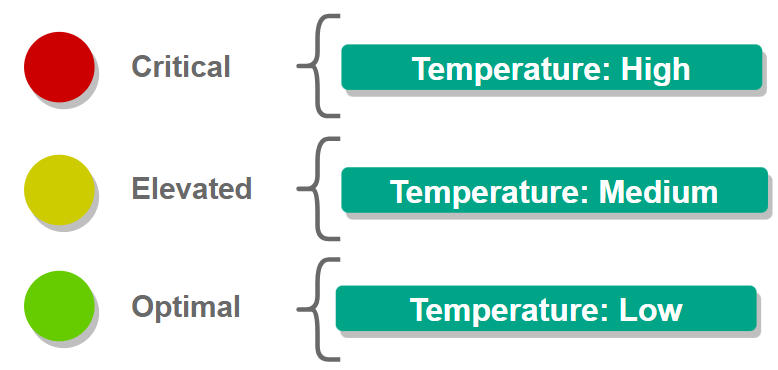
\includegraphics[width=0.6\textwidth]{RegelWerkMTBF.png}
        \caption{Regelwerk SystemMTBF}
        \label{fig:SystemMTBF}
    \end{figure}
\end{center}
\vspace{-0.5cm}
%Steht der eingang auf \textit{Low} wird der Ausgang auf \textit{Optimal} gesetzt. Steht der Eingang auf \textit{Medium}, wird der Ausgang auf \textit{Elevated} gestezt. Steht der Eingang auf \textit{High}, wird der Ausgang auf \textit{Elevated} gesetzt. Das Ergebnis wird in der \textit{SystemMTBF} Tabelle der Datenbank gespeichert. (Siehe Abbildung \ref{fig:DBModellErweitert})  

Der Algorithmus ist in ablaufdiagremm \ref{}
\begin{center}
    \begin{figure}[h!]
        \centering
        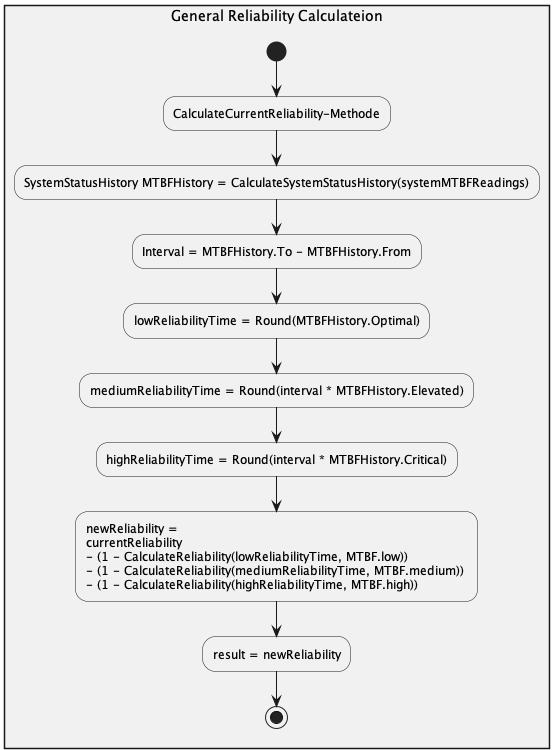
\includegraphics[width=0.5\textwidth]{SystemReliabilityBerechnungL.png}
        \caption{}
        \label{}
    \end{figure}
\end{center}
\vspace{-0.5cm}


\subsubsection*{Klassenarchitektur}
Da die Algorithmen zur berechnen der Systemstatus Historie so wie der Reliability des Systems unabhängig von Hardwarekonfiguration sind, wird das Verzeichnis \textit{HM.ScoringModel} um die, in Abbildung \ref{fig:SystemHistoryWrapper} abgebildete, \textit{StatusHistory} Klasse erweitert. Dieses bietet Zwei Funktinoen, mit welchen die Systemzuverlässigkeit so wie die SystemStatusHistorie berechnet werden kann. Da Lediglich die temperaturabhängigen \ac{mtbf} werte der Zielplatformen sich unterscheiden können, sollen diese beim Aufruf der Funktion \textit{CalculateCurrentReliability} übergeben. 
\begin{center}
    \begin{figure}[h!]
        \centering
        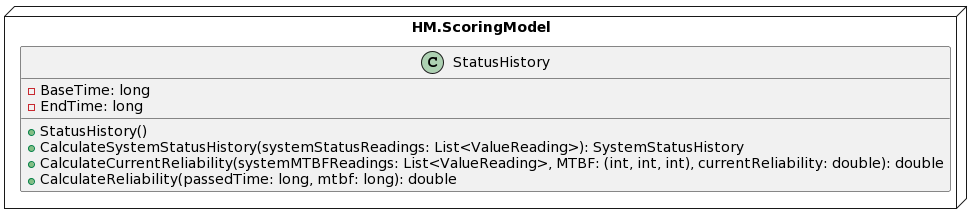
\includegraphics[width=1\textwidth]{StatusHistory.png}
        \caption{Wrapperklasse zur berechnung von Reliability und der Systemstatus Historie}
        \label{fig:SystemHistoryWrapper}
    \end{figure}
\end{center}
\vspace{-0.5cm}
